\documentclass{standalone}
\usepackage{tikz}
\usetikzlibrary{patterns, positioning}


\begin{document}
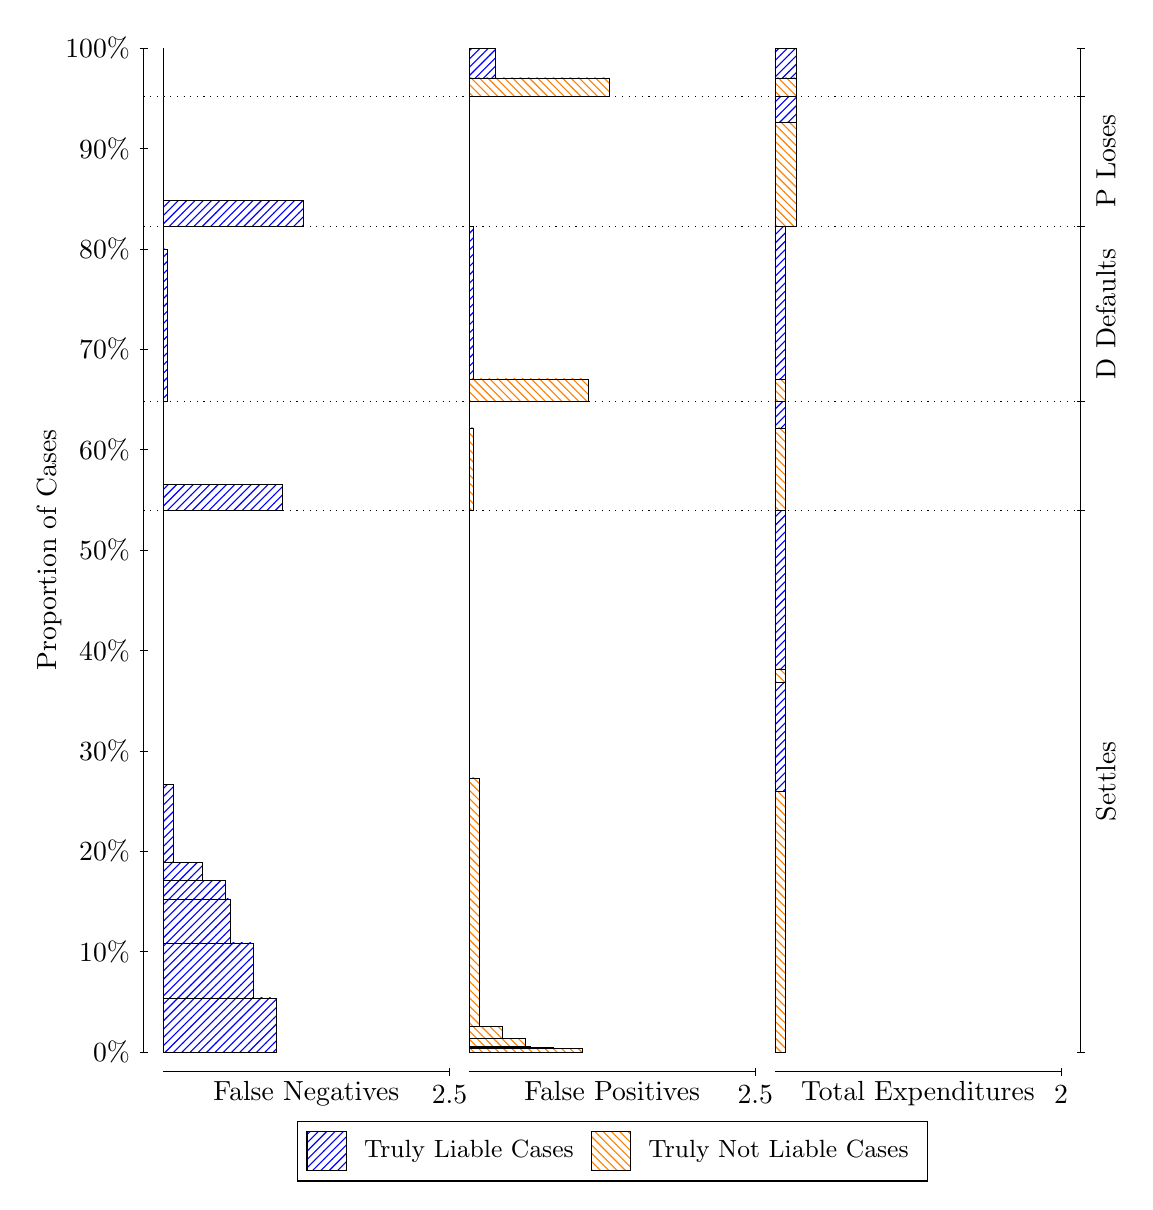
\begin{tikzpicture}
\draw[black, very thin] (1.5,1.75) -- (1.5,14.5);
\node[rotate=90, text=black, anchor=center] at (0.3, 8.125) {Proportion of Cases};
\draw[black, very thin] (1.45,1.75) -- (1.55,1.75);
\node[text=black, anchor=east] at (1.45, 1.75) {0\%};
\draw[black, very thin] (1.45,3.025) -- (1.55,3.025);
\node[text=black, anchor=east] at (1.45, 3.025) {10\%};
\draw[black, very thin] (1.45,4.3) -- (1.55,4.3);
\node[text=black, anchor=east] at (1.45, 4.3) {20\%};
\draw[black, very thin] (1.45,5.575) -- (1.55,5.575);
\node[text=black, anchor=east] at (1.45, 5.575) {30\%};
\draw[black, very thin] (1.45,6.85) -- (1.55,6.85);
\node[text=black, anchor=east] at (1.45, 6.85) {40\%};
\draw[black, very thin] (1.45,8.125) -- (1.55,8.125);
\node[text=black, anchor=east] at (1.45, 8.125) {50\%};
\draw[black, very thin] (1.45,9.4) -- (1.55,9.4);
\node[text=black, anchor=east] at (1.45, 9.4) {60\%};
\draw[black, very thin] (1.45,10.675) -- (1.55,10.675);
\node[text=black, anchor=east] at (1.45, 10.675) {70\%};
\draw[black, very thin] (1.45,11.95) -- (1.55,11.95);
\node[text=black, anchor=east] at (1.45, 11.95) {80\%};
\draw[black, very thin] (1.45,13.225) -- (1.55,13.225);
\node[text=black, anchor=east] at (1.45, 13.225) {90\%};
\draw[black, very thin] (1.45,14.5) -- (1.55,14.5);
\node[text=black, anchor=east] at (1.45, 14.5) {100\%};

\draw[black, very thin] (13.4,1.75) -- (13.4,14.5);
\draw[black, very thin] (13.35,1.75) -- (13.45,1.75);
\node[anchor=west] at (13.35, 1.75) {};
\draw[black, very thin] (13.35,8.6286) -- (13.45,8.6286);
\node[anchor=west] at (13.35, 8.6286) {};
\draw[black, very thin] (13.35,10.01) -- (13.45,10.01);
\node[anchor=west] at (13.35, 10.01) {};
\draw[black, very thin] (13.35,12.238) -- (13.45,12.238);
\node[anchor=west] at (13.35, 12.238) {};
\draw[black, very thin] (13.35,13.887) -- (13.45,13.887);
\node[anchor=west] at (13.35, 13.887) {};
\draw[black, very thin] (13.35,14.5) -- (13.45,14.5);
\node[anchor=west] at (13.35, 14.5) {};

\draw[black, very thin, pattern color=blue, pattern=north east lines] (1.75,1.75) rectangle (3.1852,2.436);
\draw[black, very thin, pattern color=blue, pattern=north east lines] (1.75,2.436) rectangle (2.8945,3.135);
\draw[black, very thin, pattern color=blue, pattern=north east lines] (1.75,3.135) rectangle (2.6038,3.6952);
\draw[black, very thin, pattern color=blue, pattern=north east lines] (1.75,3.6952) rectangle (2.5312,3.9288);
\draw[black, very thin, pattern color=blue, pattern=north east lines] (1.75,3.9288) rectangle (2.2405,4.1593);
\draw[black, very thin, pattern color=blue, pattern=north east lines] (1.75,4.1593) rectangle (1.8772,5.1482);
\draw[black, very thin, pattern color=orange, pattern=north west lines] (1.75,5.1482) rectangle (1.75,8.6286);
\draw[black, very thin, pattern color=blue, pattern=north east lines] (1.75,8.6286) rectangle (3.2578,8.9624);
\draw[black, very thin, pattern color=orange, pattern=north west lines] (1.75,8.9624) rectangle (1.75,10.01);
\draw[black, very thin, pattern color=blue, pattern=north east lines] (1.75,10.01) rectangle (1.8045,11.949);
\draw[black, very thin, pattern color=orange, pattern=north west lines] (1.75,11.949) rectangle (1.75,12.238);
\draw[black, very thin, pattern color=blue, pattern=north east lines] (1.75,12.238) rectangle (3.5303,12.563);
\draw[black, very thin, pattern color=orange, pattern=north west lines] (1.75,12.563) rectangle (1.75,13.887);
\draw[black, very thin, pattern color=orange, pattern=north west lines] (1.75,13.887) rectangle (1.75,14.121);
\draw[black, very thin, pattern color=blue, pattern=north east lines] (1.75,14.121) rectangle (1.75,14.5);
\draw[black, very thin, pattern color=orange, pattern=north west lines] (5.6333,1.75) rectangle (7.0685,1.7946);
\draw[black, very thin, pattern color=orange, pattern=north west lines] (5.6333,1.7946) rectangle (6.7052,1.806);
\draw[black, very thin, pattern color=orange, pattern=north west lines] (5.6333,1.806) rectangle (6.4145,1.8188);
\draw[black, very thin, pattern color=orange, pattern=north west lines] (5.6333,1.8188) rectangle (6.3418,1.9215);
\draw[black, very thin, pattern color=orange, pattern=north west lines] (5.6333,1.9215) rectangle (6.0512,2.0761);
\draw[black, very thin, pattern color=orange, pattern=north west lines] (5.6333,2.0761) rectangle (5.7605,5.2304);
\draw[black, very thin, pattern color=blue, pattern=north east lines] (5.6333,5.2304) rectangle (5.6333,8.6286);
\draw[black, very thin, pattern color=orange, pattern=north west lines] (5.6333,8.6286) rectangle (5.6878,9.6766);
\draw[black, very thin, pattern color=blue, pattern=north east lines] (5.6333,9.6766) rectangle (5.6333,10.01);
\draw[black, very thin, pattern color=orange, pattern=north west lines] (5.6333,10.01) rectangle (7.1412,10.299);
\draw[black, very thin, pattern color=blue, pattern=north east lines] (5.6333,10.299) rectangle (5.6878,12.238);
\draw[black, very thin, pattern color=orange, pattern=north west lines] (5.6333,12.238) rectangle (5.6333,13.563);
\draw[black, very thin, pattern color=blue, pattern=north east lines] (5.6333,13.563) rectangle (5.6333,13.887);
\draw[black, very thin, pattern color=orange, pattern=north west lines] (5.6333,13.887) rectangle (7.4137,14.121);
\draw[black, very thin, pattern color=blue, pattern=north east lines] (5.6333,14.121) rectangle (5.9603,14.5);
\draw[black, very thin, pattern color=orange, pattern=north west lines] (9.5167,1.75) rectangle (9.6529,5.0589);
\draw[black, very thin, pattern color=blue, pattern=north east lines] (9.5167,5.0589) rectangle (9.6529,6.4439);
\draw[black, very thin, pattern color=orange, pattern=north west lines] (9.5167,6.4439) rectangle (9.6529,6.6154);
\draw[black, very thin, pattern color=blue, pattern=north east lines] (9.5167,6.6154) rectangle (9.6529,8.6286);
\draw[black, very thin, pattern color=orange, pattern=north west lines] (9.5167,8.6286) rectangle (9.6529,9.6766);
\draw[black, very thin, pattern color=blue, pattern=north east lines] (9.5167,9.6766) rectangle (9.6529,10.01);
\draw[black, very thin, pattern color=orange, pattern=north west lines] (9.5167,10.01) rectangle (9.6529,10.299);
\draw[black, very thin, pattern color=blue, pattern=north east lines] (9.5167,10.299) rectangle (9.6529,12.238);
\draw[black, very thin, pattern color=orange, pattern=north west lines] (9.5167,12.238) rectangle (9.7892,13.563);
\draw[black, very thin, pattern color=blue, pattern=north east lines] (9.5167,13.563) rectangle (9.7892,13.887);
\draw[black, very thin, pattern color=orange, pattern=north west lines] (9.5167,13.887) rectangle (9.7892,14.121);
\draw[black, very thin, pattern color=blue, pattern=north east lines] (9.5167,14.121) rectangle (9.7892,14.5);
\draw[black, dotted] (1.5,8.6286) -- (13.4,8.6286);
\draw[black, dotted] (1.5,10.01) -- (13.4,10.01);
\draw[black, dotted] (1.5,12.238) -- (13.4,12.238);
\draw[black, dotted] (1.5,13.887) -- (13.4,13.887);
\draw[black, very thin] (1.75,1.5) -- (5.3833,1.5);
\node[text=black, anchor=north] at (3.5667, 1.5) {False Negatives};
\draw[black, very thin] (5.3833,1.45) -- (5.3833,1.55);
\node[text=black, anchor=north] at (5.3833, 1.45) {2.5};

\draw[black, very thin] (5.6333,1.5) -- (9.2667,1.5);
\node[text=black, anchor=north] at (7.45, 1.5) {False Positives};
\draw[black, very thin] (9.2667,1.45) -- (9.2667,1.55);
\node[text=black, anchor=north] at (9.2667, 1.45) {2.5};

\draw[black, very thin] (9.5167,1.5) -- (13.15,1.5);
\node[text=black, anchor=north] at (11.333, 1.5) {Total Expenditures};
\draw[black, very thin] (13.15,1.45) -- (13.15,1.55);
\node[text=black, anchor=north] at (13.15, 1.45) {2};

\node[text=black, centered, rotate=90] at (13.72, 5.1893) {Settles};

\node[text=black, centered, rotate=90] at (13.72, 11.124) {D Defaults};
\node[text=black, centered, rotate=90] at (13.72, 13.063) {P Loses};


\draw (7.449999999999999,1.5) node[draw=none] (baseCoordinate) {};
\begin{scope}[align=center]
        \matrix[scale=0.5, draw=black, below=0.5cm of baseCoordinate, nodes={draw}, column sep=0.1cm]{
            \node[rectangle, draw, minimum width=0.5cm, minimum height=0.5cm, pattern color=blue, pattern=north east lines] {}; &
            \node[draw=none, font=\small, text=black] (B) {Truly Liable Cases}; &
            \node[rectangle, draw, minimum width=0.5cm, minimum height=0.5cm, pattern color=orange, pattern=north west lines] {}; &
            \node[draw=none, font=\small, text=black] (B) {Truly Not Liable Cases}; \\
            };
\end{scope}

\end{tikzpicture}
\end{document}